
\chapter {Policy}

La Policy sulla Sicurezza Informatica è quel documento nel quale sono
contenute tutte le
disposizioni, comportamenti e misure organizzative richieste ai dipendenti
e/o collaboratori
aziendali per contrastare i rischi informatici. Si va a identificare tutte
quelle regole che possono
essere stabilite su un Server così che le workstation collegate vengano
"controllate" nella stessa
maniera e per fare in modo che su di esse siano presenti le stesse
caratteristiche.
L'obiettivo è quello di garantire i tre goal della Sicurezza:
confidenzialità, integrità e disponibilità.
Il compito della policy è quello di stabilire cosa è permesso e cosa non
lo è, cioè distinguere cosa è
reputato sicuro (e quindi autorizzato) da cosa invece può portare ad una
violazione del sistema. Il
sistema si muove da uno stato ad un altro. Ciò che deve fare la policy è
fare in modo che questo
non assuma mai in stati non sicuri. Un sistema si dice “sicuro” quando ciò
non accade mai.
Quando un sistema permette ad un utente o ad un processo di entrare in uno
stato non autorizzato
si dice che si è verificato un “security breach”.
Sia X un set di entità e I un informazione:
\begin{itemize}
      \item I ha confidenzialità con rispetto a X se nessun membro di X può
            ottenere alcuna
            informazione su I;
      \item I ha integrità con rispetto a X se tutti i membri di X si fidano
            di I. Le nozioni di “fiducia” e
            “integrità” sono collegate. Se un sistema ha integrità, dobbiamo
            fidarci del fatto che il suo
            comportamento è corretto. Se I è una risorsa, la sua integrità implica
            che essa funzioni
            come dovrebbe (assurance);
      \item I ha disponibilità con rispetto a X se tutti i membri di X hanno
            accesso ad I.
\end{itemize}


\paragraph{Confidentiality Policy.}

Il suo scopo è garantire che tutto lo staff comprenda i requisiti
dell'organizzazione in relazione alla
divulgazione di dati personali e informazioni riservate.
Riguardo al flusso delle informazioni è possibile possedere diversi
diritti. Si può, infatti:
\begin{itemize}
      \item Trasferire i diritti di accesso;
      \item Trasferire le informazioni senza però trasferire i diritti;
      \item Avere diritto di accesso alle informazioni solo per un certo
            periodo di tempo.
\end{itemize}

Il modello della policy spesso dipende dalla fiducia.

\paragraph{Integrity Policy.}

Definisce come l'informazione può essere modificata o alterata.
Specifica:
\begin{itemize}
      \item Chi può effettivamente compiere queste operazioni;
      \item Sotto quali condizioni i dati possono essere alterati;
      \item Eventuali limiti sulle modifiche dei dati.
\end{itemize}

Un mezzo per ottenere l'integrità è la separazione dei compiti.
Si deve fare in modo che tutte le operazioni compiute (transazioni) mantengano il sistema in uno
stato “consistente”.

\paragraph{Availability.}

Tipi di disponibilità:
\begin{itemize}
      \item Tradizionale: x ha o no l'accesso;
      \item Quality of Service: viene promesso un certo livello di accesso
            che però non è garantito (ad esempio, un livello
            specifico di larghezza di banda).
\end{itemize}

\paragraph{La policy e i suoi meccanismi: }
La policy descrive ciò che è permesso e cosa no, i meccanismi,
invece, controllano come questa viene implementata. Chiaramente gli utenti devono verificarsi
della policy, ma anche dei meccanismi utilizzati.
Le policy prese in considerazione per il controllo sugli accessi sono:
\begin{itemize}
      \item Discretionary Access Control (DAC): il proprietario determina i diritti di accesso.
            Solitamente sono identity-based access control (IBAC), ovvero il proprietario indica anche
            quali altri utenti possono avere l'accesso;
      \item Mandatory Access Control (MAC): policy più restrittive. Stabiliscono a priori quali sono i
            comportamenti da evitare e quelli permessi. Ciò non viene specificato da chi crea la risorse,
            ma anche dalle regole generali che vengono messe in atto, per esempio quelle aziendali;
      \item Originator Controlled Access Control (ORCON): policy dove colui che assegna i diritti è il
            creatore. I possessori dei file non detengono diritti e non possono cederli a loro volta;
      \item Role Based Access Control (RBAC): usate in ambito commerciale per la gestione delle
            risorse a livello amministrativo e aziendale.
            Quando si definisce una policy si devono sempre tenere presenti:
      \item Gli utenti;
      \item I ruoli che essi ricoprono: utente, utente segreto, sistemista, utente negligente..
      \item Le operazioni che possono essere compiute o no: leggere, scrivere, “downgrade”, cambio
            password...
      \item Le modalità con cui vietare o consentire determinate operazioni: obbligo, permesso, divieto,
            discrezionalità..
\end{itemize}

\section{Confidentiality Policies}
Una politica di riservatezza, chiamata anche “information flow policy”,
impedisce la divulgazione
non autorizzata di informazioni. Il suo obiettivo è quello di specificare quali
dati devono essere
protetti e da chi o da che cosa vanno protetti. In poche parole, indicano un
insieme di principi e
regole che definiscono i possibili accessi al sistema.

Distinguiamo tra:

\begin{itemize}
      \item \textbf{Oggetti:} una qualunque entità passiva che necessita di
            essere protetta;
      \item \textbf{Soggetti:} una qualunque entità attiva che può manipolare
            gli oggetti (persone o processi).
\end{itemize}

Un modello di sicurezza definisce i soggetti, gli oggetti ai quali i soggetti
hanno accesso ed i diritti
di accesso, che non sono altro che le operazioni con le quali è possibile
operare. Un soggetto può
avere diritti di accesso sia per gli oggetti che per altri soggetti.
Esistono due tipi di modelli di sicurezza:
\begin{itemize}
      \item \textit{Discretionary access control} (\textbf{DAC}): meccanismo
            attraverso il quale gli utenti possono
            liberamente decidere di garantire o revocare l'accesso a determinati
            oggetti.
            \begin{itemize}
                  \item Gli utenti amministrano i dati che possiedono (vengono
                        detti proprietari);
                  \item Il proprietario può autorizzare altri utenti all'accesso;
                  \item Il proprietario può definire il tipo di accesso da
                        concedere agli altri;
                  \item Accessi selettivi.
            \end{itemize}
      \item \textit{Mandatory access control} (\textbf{MAC}): meccanismo
            attraverso il quale le decisioni di accesso
            sono basate su delle etichette che contengono informazioni
            rilevanti alla sicurezza di un
            oggetto. Questo metodo fornisce l'accesso alla risorsa in base al
            livello di autorizzazione dell'utente.
            \begin{itemize}
                  \item Classificazione dei dati (livelli di sensibilità);
                  \item Classificazione dei soggetti (autorizzazione);
                  \item Classe di sicurezza <componente gerarchica, insiemi di
                        categoria>;
                  \item Ordinamento (parziale) tra le classi di sicurezza;
                  \item I meccanismi di sicurezza devono garantire che tutti i
                        soggetti abbiano accesso solo
                        ai dati per cui possiedono le autorizzazioni appropriate;
                  \item Non si possono propagare privilegi.
            \end{itemize}
\end{itemize}

\subsection{Modello Bell-LaPadula}
È un modello tipico \textbf{MAC}. Fu proposto da Bell-LaPadula nel 1976 con lo scopo di
rafforzare i
controlli ai possibili accessi alle applicazioni militari (corrisponde, infatti,
alle classificazioni
stile-militare). Viene anche chiamato modello “\textit{a multi-livelli}”.
Nelle applicazioni i soggetti e gli oggetti vengono partizionati in differenti
livelli di sicurezza. Un
soggetto può solo accedere ad oggetti a certi livelli, i quali dipendono
strettamente dal loro
livello di sicurezza. Per esempio, i seguenti sono due tipici specificazioni di
accessi: “una persona
\verb|UNCLASSIFIED| non può leggere informazioni a livello \verb|CONFIDENTIAL|” e
“informazioni \verb|TOP SECRET| non possono essere scritte in files di livello
\verb|UNCLASSIFIED|”.
Gli oggetti sono classificati in 4 diversi livelli di sensibilità, cioè di
confidentiality. Ciascun oggetto
può essere associato a uno o più livelli, detti compartments.
Ad ogni soggetto, invece, viene associata una “\textit{clearance}” ovvero
un'autorizzazione. Una
clearance non è altro che una coppia del tipo \verb|<rank, compartments>|
dove \verb|rank| è il massimo livello di sensibilità dell'informazione a cui
il soggetto ha accesso; \verb|compartment| indica i comparti a
cui il soggetto può accedere.
A tutte le entità vengono assegnati dei livelli di sicurezza. In particolare:

\begin{itemize}
      \item Un soggetto S possiede “\textit{security clearance}” \(L(S)=l_s\);
      \item Un oggetto O possiede “\textit{security classification}” \(L(O)=l_o\);
\end{itemize}

Per ogni classificazione di sicurezza \(l_i, \ i=0,...,k-1 \ con \ l_i<l_i+1\),
quindi i livelli di sicurezza sono
disposti in ordine lineare.
Il tipo più semplice di classificazione della confidenzialità è un insieme di
autorizzazioni poste in
gerarchia: \verb|Top secret > Secret > Confidential > Unclassified|.
Il modello definisce due regole obbligatorie del controllo accessi (MAC):
\begin{itemize}
      \item \textbf{Simple Security Condition:} S può leggere O se e solo se
            \(l_o \le l_s\) e S ha discrezione
            nell'accesso in lettura a O. Questa regola viene anche detta “No Read Up”
            e impedisce ai
            soggetti di leggere oggetti a livelli superiori. Il proprietario può
            aggiungere anche dei diritti di
            tipo DAC, ovvero può restringere ulteriormente l'accesso.
      \item \textbf{* Property} (Star property): S può scrivere su O se e solo
            se \(l_s \le l_o\) e S ha discrezione
            nell'accesso alla scrittura su O. La regola è anche detta “No Write Down”
            e impedisce ai
            soggetti di scrivere su oggetti di livello inferiore. Questo perché se no
            un utente potrebbe declassificare
            informazioni o oggetti scrivendoli all'interno di oggetti con grado di
            classificazione inferiore.
\end{itemize}

Si potrebbe estendere il modello addizionando un gruppo di categorie per ogni
classificazione di
sicurezza. Ogni categoria descrive un tipo di informazioni.
Tali categorie risultano dal principio del “Need To know”: limito l'accesso alle
sole informazioni per
le quali l'utente ha necessità di accedere.

\paragraph{Esempio:} %% TODO: ricontrollare foto e scritte, queste non coincidono
CATEGORIE \(\rightarrow\) NUC, EUR e US
Ogni soggetto ha un'autorizzazione ad un determinato livello di sicurezza e può
accedere anche
ad alcuni dei livelli inferiori.

\begin{figure}[H]
      \centering
      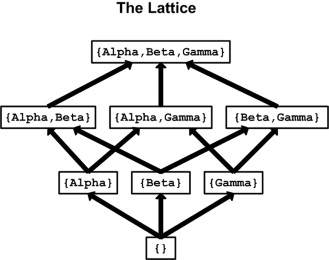
\includegraphics[width=8cm, keepaspectratio]{capitoli/policy/imgs/Lattuce.jpg}
\end{figure}

\subsection{Multilevel Security}
Il concetto viene trattato per la prima volta nel “Red Book”nel 1987.
La sicurezza multilivello o più livelli di sicurezza (\textbf{MLS}) è
l'applicazione di un sistema di computer
per elaborare le informazioni con incompatibili classificazioni (cioè, a diversi
livelli di sicurezza),
consentire l'accesso da parte di utenti con diversi spazi di sicurezza e le
esigenze di sapere (need
to know) e impedire agli utenti di ottenere l'accesso alle informazioni per
le quali non hanno
l'autorizzazione.
La sicurezza multilivello viene implementata in ambiti particolari, dove è
necessario un controllo
obbligatorio degli accessi, per assicurare che le politiche di sicurezza siano
garantite dal sistema.
L'ente definisce delle regole in merito a chi può accedere e anche a che cosa;
queste regole non
possono essere modificate dai singoli utenti.
I sistemi MLS ci assicurano diversi livelli di sicurezza L che definiscono la
classificazione dei
soggetti (processi) e degli oggetti. I livelli di affidabilità, cioè di
“assurance”, vengono stabiliti in
base a vari criteri di valutazione:
\[
      (worst) \ D<C1<C2<C3<B1<B2<B3<A1 \ (best)
\]
In base ai dati e alle circostanze possono essere richiesti livelli più o meno
elevati. Solitamente, in
presenza di un solo livello, è sufficiente una macchina del tipo C2 o C3. Da B1
in poi, invece, si
possono gestire efficacemente informazioni su livelli multipli.
\begin{center}
      \begin{tabular}{ |c|c| }
            \hline
            \textbf{System Stores}   & \textbf{Minimum Assurance} \\
            \hline
            TopSecret + Unclassified & B3                         \\
            \hline
            TopSecret + Secret       & B2                         \\
            \hline
            Secret + Unclassified    & B1                         \\
            \hline
      \end{tabular}
\end{center}
TopSecret+Unclassified rappresentano in realtà 3 livelli, insieme al Secret.
Attaccare una macchina B3 costa certamente di più che attaccare B1 o B2.

\subsubsection{Configurazione di reti MLS: Channel Cascade Attacks}     %% TODO: troppo lungo rompe l'indice
Prendiamo in esame la seguente immagine:
\begin{figure}[H]
      \centering
      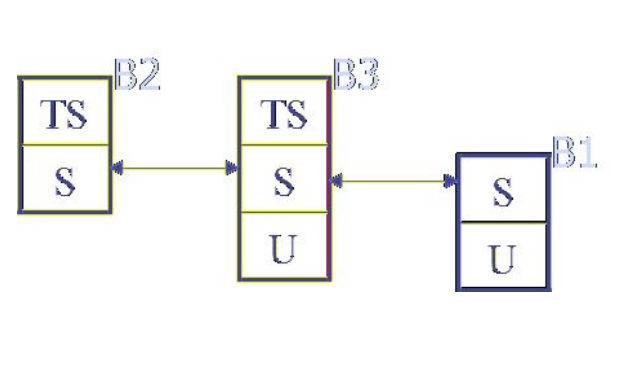
\includegraphics[width=8cm, keepaspectratio]{capitoli/policy/imgs/cascade1.png}
\end{figure}
I livelli di sicurezza delle macchine sono B1, B2 e B3. Lo
sforzo (l'effort) viene effettuato da un attaccante, il quale
cerca di penetrare una macchina con un determinato livello
di sicurezza.
Il “\textbf{cascade attack}” si ha quando una sola macchina viene attaccata ad
un certo livello, ma anche
le altre vengono coinvolte conseguentemente.
L'informazione tra i sistemi è condivisa, quindi può fluire tra le macchine.
Nell'esempio, infatti, sono
tutte collegate a livello S. Grazie all'effort su B2 si riesce a portare
l'informazione da TS a U, che
equivale a dire di aver buttato giù un sistema B3. Quindi, a partire da B2,
si riesce a buttar giù
anche B1 e B3.
Si dice “attacco a cascata” perché grazie ad uno sforzo relativamente piccolo
(nel nostro caso
effettuato su B2) si possono attaccare anche sistemi più grandi e sicuri,
poiché sono interconnessi.
In generale quindi, se l'attacco ha successo, il livello di segretezza può
essere abbassato da
TopSecret a Secret, fino a Unclassified.
Si ha un “cascading attack” se esiste un “cascading path”, ovvero un cammino
tra sistemi che
costa meno dello sforzo necessario a rompere i singoli sistemi.
Ricordiamo che eliminare i cascade path è un problema che rientra in NP.

\paragraph{Come eliminate il Cascade Path}
\begin{itemize}
      \item  Si possono disconnettere le macchine. Più c'è condivisione,
            più si alza la possibilità di
            avere cascading path;
      \item  Mettere in comunicazione le macchine a livelli diversi;
      \item  Definire i flussi consentiti (ognuno avrà uno specifico costo).
\end{itemize}
Il seguente non è un cascading path (non va bene perché dovremmo
rompere un sistema B3. L'effort è uguale all'attacco, non c'è il
guadagno).
\begin{figure}[H]
      \centering
      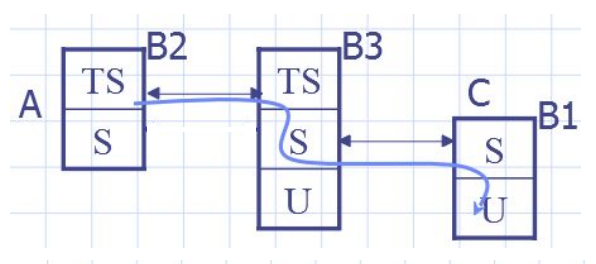
\includegraphics[width=8cm, keepaspectratio]{capitoli/policy/imgs/cascade3.png}
\end{figure}
Questo invece è un cascading path (quando il livello dell'attacco è più
grande dello sforzo).
\begin{figure}[H]
      \centering
      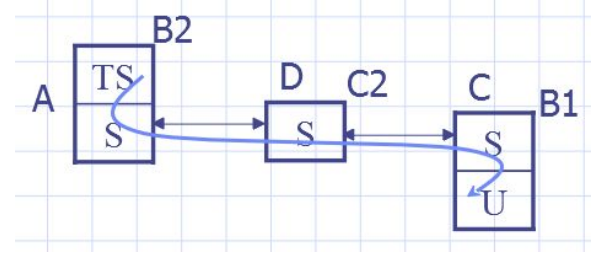
\includegraphics[width=8cm, keepaspectratio]{capitoli/policy/imgs/cascade2.png}
\end{figure}

\subsection{Secure Interoperation}

\begin{figure}[H]
      \centering
      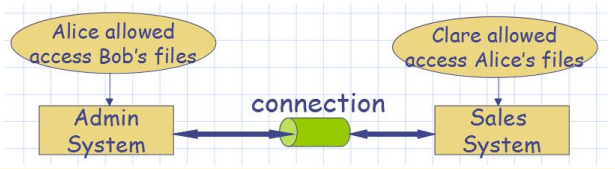
\includegraphics[width=10cm, keepaspectratio]{capitoli/policy/imgs/secure_interoperation.png}
\end{figure}

Supponiamo di avere due sistemi all'interno ad un'azienda, uno per le Vendite e
uno per
l'Amministrazione. Ognuno ha la propria policy che chiaramente definisce i
diritti degli utenti.
Alice lavora su entrambi i sistemi e vorrebbe che i filesystem venissero
connessi (I sistemi sono
sicuri individualmente). Se ciò avvenisse, allora anche Clare avrebbe accesso
ai file dell'Admin
System. Ciò rappresenta a tutti gli effetti un attacco al sistema.

Le possibili soluzioni sono:

\begin{itemize}
      \item Togliere a Clare l'accesso ai file di Alice;
      \item togliere ad Alice l'accesso ai file di Bob.
\end{itemize}

In generale quindi è necessario riconfigurare il sistema in modo da eliminare
alcune connessioni e
di conseguenza ridurre i diritti degli utenti.

\subsection{Access Interoperation}

\begin{figure}[H]
      \centering
      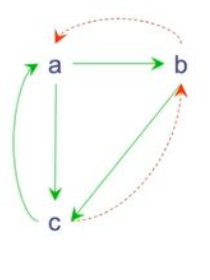
\includegraphics[width=4cm, keepaspectratio]{capitoli/policy/imgs/access_interoperation.png}
\end{figure}

Consideriamo la figura precedente che ci mostra una policy (rappresentata dalle
linee verdi) la quale definisce i seguenti accessi.
L'accesso da \verb|A| a \verb|C| potrebbe essere ottenuto per transitività
passando per \verb|B|.
Stesso discorso vale per \verb|C| e \verb|B|: da \verb|C| si può arrivare a
\verb|B| tramite \verb|A|. Ma il fatto che
da \verb|C| si possa raggiungere \verb|B| viola la policy, perché questo accesso
non è definito in realtà. \'{E} necessario quindi riconfigurare il sistema.
Eventuali soluzioni potrebbero essere:
\begin{itemize}
      \item Esplicitare i flussi, quindi ciò che è effettivamente permesso e
            cosa non lo
            è (ovvero aggiungere anche le linee rosse);
      \item Esplicitare soltanto ciò che è vietato (linee rosse) e quindi il
            resto è default permit;
      \item Esplicitare soltanto ciò che è permesso (linee verdi) e quindi il
            resto è default deny.
\end{itemize}
Va ricordato che la riconfigurazione deve essere safe: ciò che viene stabilito
con la nuova
configurazione deve
essere un sottoinsieme di ciò che era permesso anche prima: non dobbiamo andare
ad escludere per errore flussi già esistenti. La policy deve essere rispettata
sempre, anche dopo la riconfigurazione.

\subsection{Secure Reconfiguration}

Supponiamo di avere due differenti policy, corrispondenti a due diversi sistemi
che devono però
interoperare. Unire le due policy potrebbe non essere così semplice, in quanto
potrebbero
verificarsi dei conflitti.
A questo punto è necessario capire a cosa dare priorità, se a ciò che è permesso
o a ciò che non lo è. Solitamente si dà priorità al default deny, altrimenti
non ci sarebbe garanzia del fatto che il sistema sia ancora safe.

\begin{figure}[H]
      \centering
      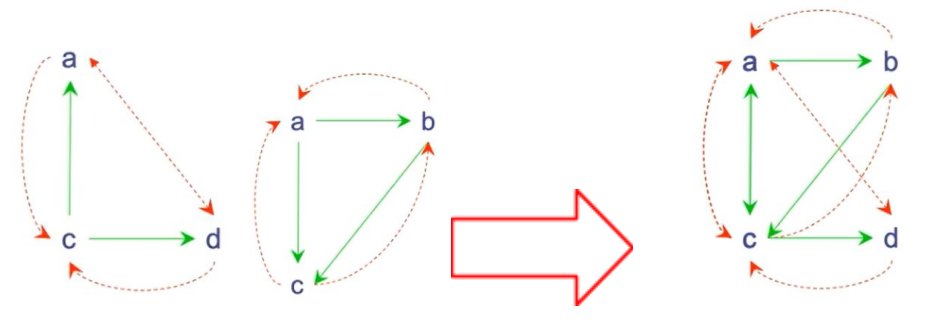
\includegraphics[width=10cm, keepaspectratio]{capitoli/policy/imgs/secure_recognition.png}
\end{figure}

Una volta esplicitato cosa è vietato, si può definire cosa è invece permesso,
assicurando il fatto
che non ci sia alcuna transitività.
Il nuovo schema della policy deve essere proiettato sui sistemi a cui è
destinato per verificare che
non si presentino comunicazioni non corrette.

\begin{figure}[H]
      \centering
      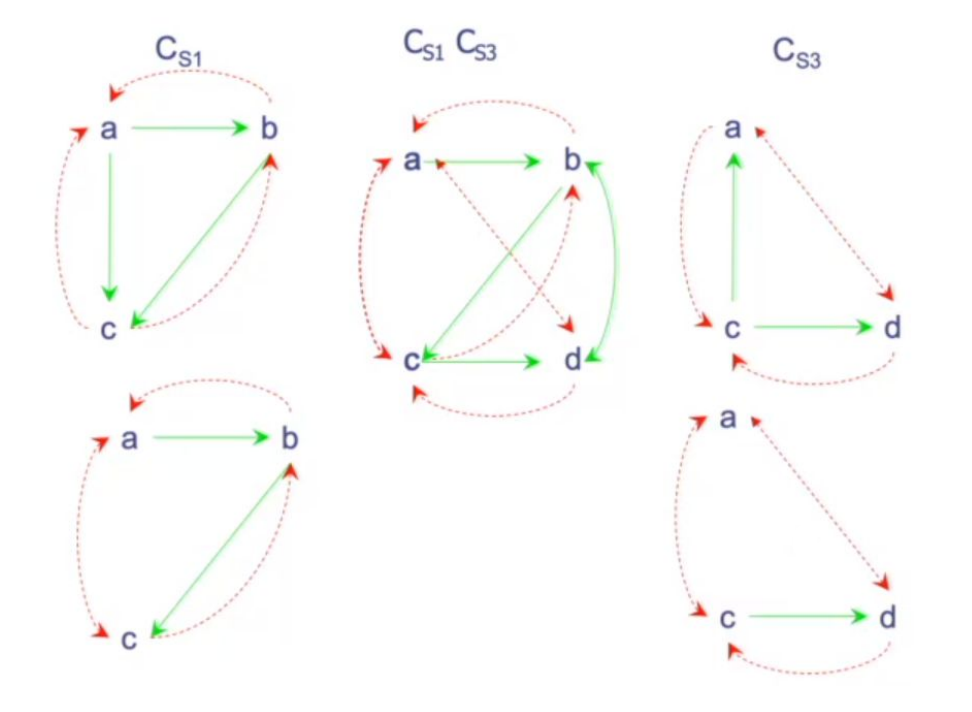
\includegraphics[width=12cm, keepaspectratio]{capitoli/policy/imgs/secure_regognition2.png}
\end{figure}

\section{Integrity Policies}
Possiamo distinguere due diversi tipi di integrità:
\begin{itemize}
      \item \textbf{Il livello di integrità di un soggetto} è una misura della
            fiducia che si ripone nella sua
            capacità di produrre o gestire informazioni. Per esempio,
            un'applicazione certificata può
            avere una maggiore integrità rispetto al freeware
            scaricato da internet.
      \item \textbf{Il livello di integrità di un oggetto} descrive il grado
            di “affidabilità” dell'informazione
            contenuta in quell'oggetto.
\end{itemize}

Una meta-policy che i modelli di integrità devono soddisfare è necessariamente
quella di non
permettere che informazioni meno affidabili corrompano quelle più affidabili.
Le informazioni con
bassa integrità non dovrebbero fluire in domini ad alta integrità.
Più alto è il livello, maggiore è la fiducia (trust). Quindi è più probabile
che:
\begin{itemize}
      \item Un programma venga eseguito correttamente;
      \item I dati siano precisi e/o affidabili.
\end{itemize}
\'{E} importante precisare che avere un alto livello di integrità non significa
avere un alto livello di
confidenzialità e viceversa.
In generale se P è un processo con un grado X di “affidabilità”
(\textbf{trustworthiness}) non può
modificare dati ad un livello più alto di lui perché è certificato solo fino
a quel punto; quindi può
modificare o scrivere informazioni nei livelli sottostanti.
I requisiti che una policy di integrità deve rispettare sono:
\begin{itemize}
      \item Gli utenti non possono usare programmi scritti da loro stessi ma
            devono usare programmi e
            DB già esistenti;
      \item Separazione delle funzioni: i programmatori sviluppano e testano
            programmi su un sistema
            diverso da quello di produzione. Quando sono richiesti dei dati in
            fase di testing, non
            vengono presi i dati reali ma dei dati opportunamente modificati
            tramite un processo
            speciale. Tali dati vengono usati solo nella fase di sviluppo e non
            in quella di produzione;
      \item Separazione dei compiti;
      \item Logging and auditing: il processo deve essere controllato,
            verificato (audited), tracciato (logging) e
            deve offrire la possibilità di effettuare un'operazione di rollback;
      \item I manager e coloro che eseguono il processo di verifica devono
            avere accesso ad entrambi
            gli stati dei sistemi ed ai log generati da essi.
\end{itemize}

\subsection{Modello BIBA}

Il modello di integrità Biba venne sviluppato per aggirare le debolezze del
modello di protezione
Bell-LaPadula, il quale non prevedeva la possibilità di eliminazione implicita
degli oggetti di
sicurezza scritti da loro.
Il modello di Biba in generale ha l'obiettivo di preservare l'integrità, ma in
particolare vuole:

\begin{itemize}
      \item Prevenire la modifica dei dati da soggetti non autorizzati;
      \item Prevenire modifiche non autorizzate ai dati da soggetti autorizzati;
      \item Mantenere la consistenza interna ed esterna (es.: dati che
            rispecchino il mondo reale).
\end{itemize}

Implementa le protezioni definendo una serie ordinata di livelli di integrità
per i soggetti e gli
oggetti, rispettando le regole:

\begin{itemize}
      \item \textbf{Read Up:} Questo significa che
            un soggetto che si trova al livello di integrità X può leggere
            solo oggetti allo stesso livello o
            superiore (“assioma di integrità semplice”);
      \item \textbf{Write Down:} un soggetto al livello di integrità X può
            scrivere solo oggetti allo stesso livello
            o di livello più basso (assioma di integrità * o Proprietà di
            semplice sicurezza);
\end{itemize}
Un esempio è quello della gerarchia militare: un generale può solo ricevere
ordini dai suoi superiori o parigrado e può imporre ordini solo ai suoi
sottoposti o parigrado per evitare un cambiamento/danneggiamento
nella missione da svolgere.
Da notare che \textit{Read Up} e \textit{Wite Down} sono l'opposto delle regole
\textit{Read Down}, \textit{Write Up} del modello Bell-LaPadula.\\

È impossibile trasformare informazioni meno trusted in più trusted.
L'obiettivo di tale modello è quello di evitare che il grado di fiducia di
un'informazione aumenti. Se ciò
si verificasse, si potrebbe considerare fidata un'informazione che in realtà
non lo è.
Ad ogni risorsa del sistema viene assegnata un'\textit{etichetta} indicante
il livello di integrità minimo
richiesto per l'accesso da parte dei soggetti. Le etichette di integrità,
non coincidono con quelle di
confidenzialità: le prime limitano le modifiche che si possono fare alle
informazioni, mentre le
seconde limitano il flusso delle informazioni. Maggiore è il livello di
integrità e maggiore è la
certezza che un programma sia eseguito correttamente e che i dati siano accurati
e veritieri.
Esistono delle relazioni tra integrità e la sua affidabilità. I livelli di
integrità sono un punto
importante per la sicurezza ma non coincidono con i livelli di sicurezza.\\

Ricordarsi che i modelli Bell-LaPadula e BIBA sono in conflitto tra loro e
non si possono utilizzare
contemporaneamente.

\subsection{Modello Clark-Wilson}

Rappresenta un'alternativa al modello di Biba ed utilizza le transazioni come
operazioni base per
garantire integrità prima e dopo le operazioni.
Si basa su questi tre principi:

\begin{itemize}
      \item \textbf{Separazione dei compiti}: Se sono necessarie due o più fasi per
            eseguire una funzione,
            almeno due persone devono eseguire le fasi separandosi adeguatamente
            i compiti;
      \item \textbf{Separazione delle funzioni}:
            \begin{itemize}
                  \item Una singola persona non può svolgere ruoli complementari
                        in un processo critico;
                  \item Gli sviluppatori non sviluppano nuovi programmi sui
                        sistemi di produzione;
                  \item Gli sviluppatori non elaborano i dati di produzione sui
                        sistemi di produzione;
            \end{itemize}
      \item \textbf{Auditing}: I sistemi commerciali sottolineano l'importanza del
            recupero e della responsabilità
            (recoverability e accountability). I sistemi vengono analizzati per
            determinare quali azioni
            hanno avuto luogo e chi è stato coinvolto.
\end{itemize}

In generale un dato si può trovare in uno stato consistente o non consistente,
in particolare si
troverà nello stato consistente o valido se soddisfa un insieme di vincoli
(definizione di integrità
secondo Clark Wilson).
I tasselli alla base del modello CW sono quindi:

\begin{itemize}
      \item \textbf{Autenticazione}: l'identità di tutti gli utenti deve essere
            autenticata correttamente;
      \item \textbf{Audit}: le modifiche devono essere tracciate (logging) per registrare ogni
            programma eseguito e da chi,
            in modo che non possa essere annullato;
      \item \textbf{Transazioni ben formate}: gli utenti manipolano i dati solo in modo
            limitato. Sono consentiti
            solo accessi legittimi;
      \item \textbf{Separazione dei compiti}: il sistema associa ad ogni utente un
            insieme di programmi che
            può eseguire. Impedisce le modifiche non autorizzate, preservando
            così l'integrità;
\end{itemize}

%TODO:Aggiungere l'esempio sul modello Clark-Wilson e riscriverlo a verso con matematica
\begin{figure}[H]
      \centering
      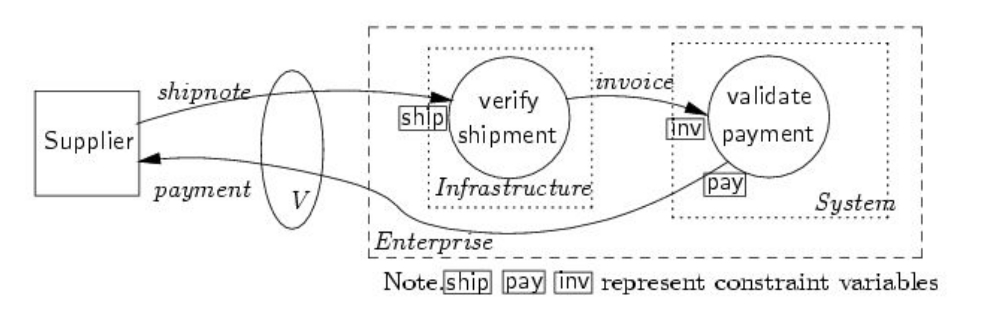
\includegraphics[width=8cm, keepaspectratio]{capitoli/policy/imgs/clark_wilson.png}
\end{figure}
\begin{figure}[H]
      \centering
      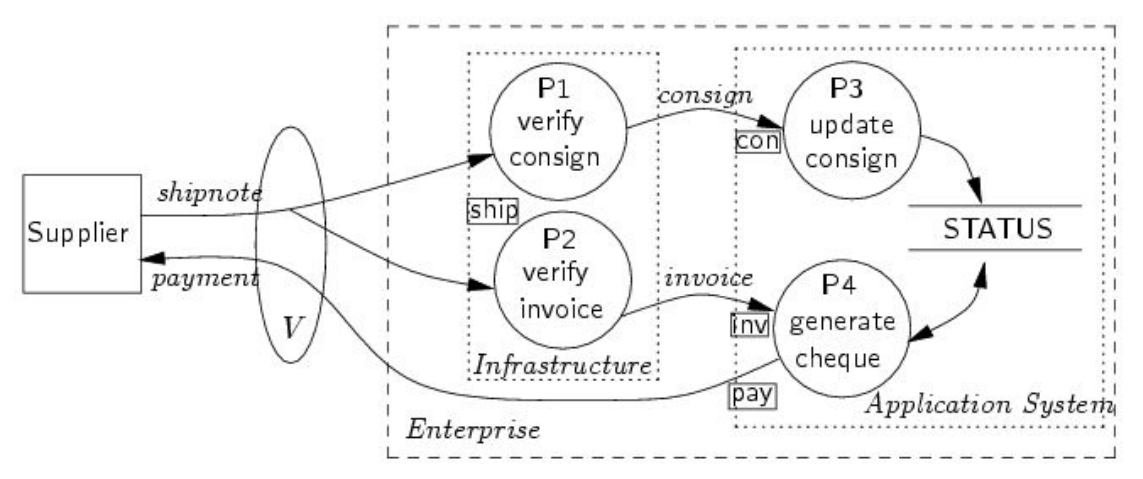
\includegraphics[width=8cm, keepaspectratio]{capitoli/policy/imgs/clark_wilson2.png}
\end{figure}

\subsubsection{Come funziona?}

Il modello Clark-Wilson è di tipo MAC e le regole sono decise dal sistema e non
dagli utenti.
Si basa su altri due concetti chiave:

\begin{itemize}
      \item Una transazione deve essere ben formata (WFT), cioè deve far passare
            il sistema da uno
            stato consistente verso altri stati consistenti. E' pertanto
            importante stabilire un
            meccanismo che permetta di esaminare e certificare che le transazioni
            siano eseguite
            correttamente;
      \item Viene rispettato il principio della separazione dei compiti:
            l'operazione viene divisa in
            sottoparti che devono essere eseguite da soggetti differenti.
            In questo modo, per attuare
            una frode, ad esempio, è necessario che tutti i soggetti delle
            transazioni ne siano
            consapevoli. In pratica vi è una distinzione tra colui che esegue
            una transazione e colui che
            la certifica.
\end{itemize}

Il modello di Clark-Wilson richiede che il Sistema Informativo, nel quale viene
applicato, disponga
delle seguenti caratteristiche essenziali:

\begin{itemize}
      \item Autenticazione da parte degli utenti;
      \item I dati possono essere manipolati da uno specifico set di procedure,
            che a loro volta
            possono essere eseguite solo da un utente autorizzato;
      \item Vengono mantenuti i log (contenenti programmi, dati e nomi degli
            utenti);
      \item I meccanismi di protezione non possono essere cambiati (staticità);
      \item Il security officer è il responsabile degli assegnamenti;
      \item Specifiche regole di sicurezza per la modifica dei dati.
\end{itemize}

\begin{figure}[H]
      \centering
      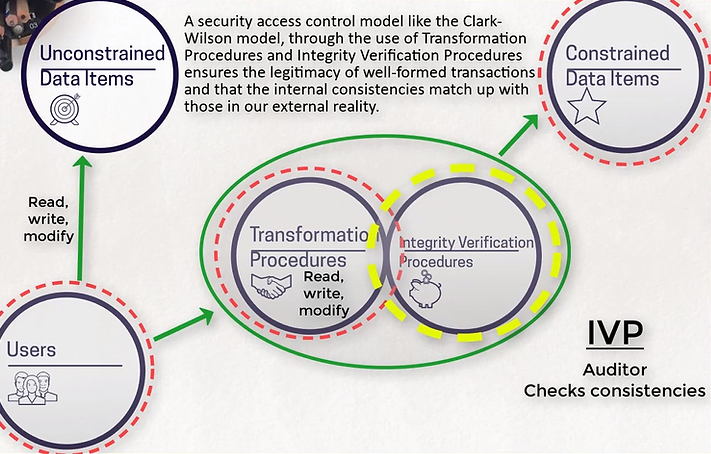
\includegraphics[width=12cm, keepaspectratio]{capitoli/policy/imgs/clark_wilson3.png}
\end{figure}

Formalmente il modello suddivide i dati in due set:

\begin{itemize}
      \item \textbf{CDI} (\textit{Constrained Data Item}): contiene gli elementi
            del sistema da proteggere, ossia i dati
            soggetti al controllo di integrità. Ad esempio in una banca, il CDI
            potrebbe essere composto
            dal saldo dei conti;
      \item \textbf{UDI} (\textit{Unconstrained Data Item}): contiene l'insieme
            dei dati non soggetti ai vincoli di
            integrità.
\end{itemize}

L'appartenenza dei dati ad una determinata classe è esclusiva.
Il modello prevede due tipi di procedure:

\begin{itemize}
      \item \textbf{IVP} (\textit{Integrity Verification Procedures}): è
            l'insieme delle funzioni che verificano se un
            determinato set di dati, appartenenti alla classe CDI, soddisfa
            determinati vincoli di
            integrità, i quali sono implementati come vincoli nel linguaggio SQL;
      \item \textbf{TP} (\textit{Transformation Procedures}): è l'insieme delle
            procedure di trasformazione che hanno in input
            ed in output dei dati appartenenti alla classe CDI. Se un set dati
            CDI di partenza soddisfa
            un determinato IVP, allora lo soddisferà anche il set CDI ottenuto
            dopo la trasformazione;
            questo risulterà vero solo se la procedura è ben formata.
\end{itemize}

Le procedure tipo IVP permettono di garantire che il sistema parta da uno stato
consistente,
mentre le procedure TP assicurano che lo stato sarà consistente anche in futuro.
Una tipica
transazione nel database è composta da TP, le quali trasformano dati UDI in CDI
oppure
aggiornano dati CDI.
Una IVP quindi garantisce che tutti i CDI nel sistema siano validi in un
determinato stato. Un TP,
invece, prende in input un CDI o un UDI e produce sempre un CDI.
Il modello utilizza le transazioni come operazioni di base. L'integrità deve
essere garantita prima e
dopo le operazioni; di conseguenza i dati possono trovarsi in uno stato coerente
oppure
inconsistente. L'integrità viene definita mediante vincoli che i dati devono
rispettare.
Definire le caratteristiche di una transazione ben formata è un lavoro manuale
eseguito da un
security officer, il quale è l'unico che può specificare il set di procedure che
possono modificare
certi CDI.

\begin{figure}[H]
      \centering
      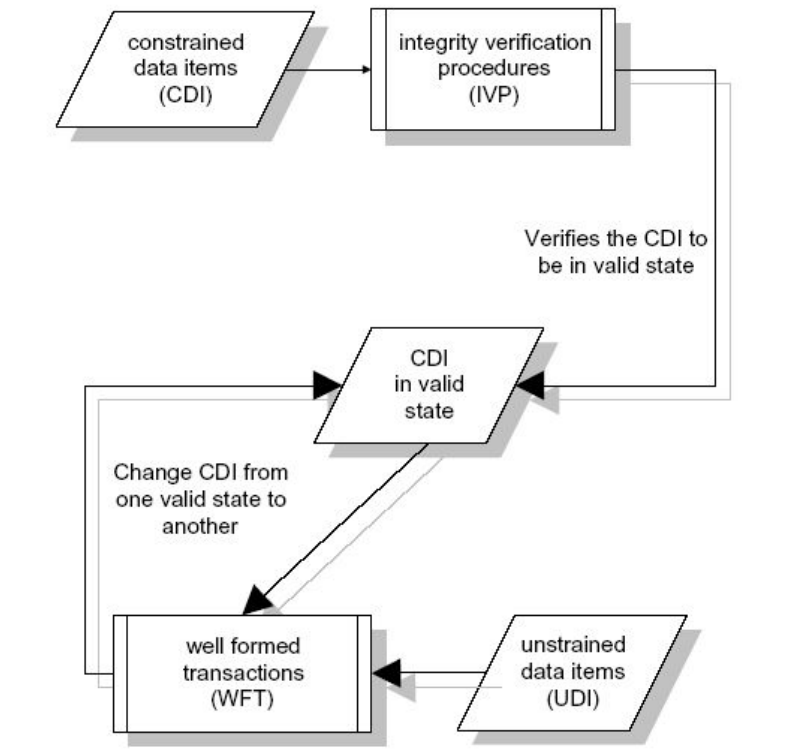
\includegraphics[width=8cm, keepaspectratio]{capitoli/policy/imgs/clark_wilson4.png}
\end{figure}

Nel caso debbano entrare nel sistema degli UDI questi devono essere processati
solo da WFT per
risultare CDI.
Il minimo di sicurezza richiesta comprende:
\begin{itemize}
      \item Integrità: i vincoli d'integrità esistono per proteggere IS da
            maligni o accidentali modifiche
            dei dati. Le regole possono essere definite su stati statici del db
            o su transazioni (es. prima
            di poter effettuare un modifica);
      \item Identificazione, autenticazione: prima di accedere a un sistema ogni
            utente deve essere
            identificato e autenticato per mantenerne traccia e per dargli
            l'accesso;
      \item Autorizzazioni (cioè controllo sugli accessi)
\end{itemize}

\subsubsection{Regole di certificazione}
Al fine di garantire la validità dei dati nel sistema, il modello di
Clark-Wilson prevede le seguenti
regole di certificazione:
\begin{itemize}
      \item \textbf{CR1} se un IVP è eseguito, deve assicurarsi che tutti i CDI
            siano in uno stato valido.
      \item \textbf{CR2} una TP deve trasformare un insieme di CDI da uno stato
            valido ad uno valido
            \begin{itemize}
                  \item CR2 definisce come “certificata” una relazione che
                        associa un insieme di CDI ad
                        una TP;
                  \item CR2 implica che una TP può corrompere una CDI se non è
                        certificata per lavorare
                        con quel CDI
                        \begin{itemize}
                              \item \textit{Esempio}: la TP che investe denaro nel
                                    portafoglio azionario della banca
                                    corromperebbe i bilanci anche se la TP
                                    fosse certificata a lavorare sul
                                    portafoglio, poiché le azioni della TP
                                    potrebbero non avere senso sui conti
                                    bancari
                              \item Da ciò nasce la prima regola di rinforzo
                        \end{itemize}
            \end{itemize}
\end{itemize}

\subsubsection{Regole di rinforzo}

Tutte le TP devono essere certificate per essere valide.
Un TP può manipolare in modo errato (cioè non conforme ad un IVP) un CDI se
non è stato
certificato a lavorare per questo. Per evitare il problema, esistono delle
regole di rinforzo
(enforcement):

\begin{itemize}
      \item \textbf{ER1} Il sistema deve garantire che solo le TP certificate ad
            operare su determinati CDI svolgano
            operazioni su di essi.
      \item \textbf{ER2} Il sistema deve associare a ciascun TP un utente e un
            insieme di CDI su cui l'utente e la TP possono lavorare. Il TP può
            accedere a quei CDI per conto dell'utente, ma non può accedere per conto di
            utenti non autorizzati.
            \begin{itemize}
                  \item Il sistema deve mantenere le relazioni certificate;
                  \item Il sistema deve restringere l'accesso degli utenti alle
                        TP mediante una relazione di
                        permesso che specifica quali utenti possono eseguire
                        certi TP e su quali CDI.
            \end{itemize}
\end{itemize}

\subsubsection{Utenti e regole}

\begin{itemize}
      \item \textbf{CR3} Le relazioni di permesso devono essere basate sulla
            separazione dei compiti.
      \item \textbf{ER3} Il sistema deve autenticare ogni utente che vuole
            utilizzare una TP.
\end{itemize}

\subsubsection{Uso dei Log}

\begin{itemize}
      \item \textbf{C4} Tutte le TP devono scrivere in CDI di solo accodamento
            (append) tutte le informazioni
            sufficienti a ricostruire le operazioni svolte.
            \begin{itemize}
                  \item Questo CDI è il log;
                  \item Gli amministratori devono essere in grado di capire
                        cosa ha fatto una determinata
                        transazione.
            \end{itemize}
\end{itemize}

\subsubsection{Trattamento di input non fidato}

\begin{itemize}
      \item \textbf{CR5} Ogni TP che prende in input un UDI può eseguire solo
            trasformazioni valide, oppure
            nessuna trasformazione, per ogni possibile valore dell'UDI.
            La trasformazione può quindi rifiutare il
            UDI o trasformarlo in un CDI.
            \begin{itemize}
                  \item Un possibile esempio: in un banca i numeri inseriti
                        da tastiera sono UDI, i quali non possono essere dati in input
                        ad una TP. Un'apposita TP deve validare tali numeri
                        (rendendoli un CDI) prima di usarli; se
                        la validazione fallisce, la TP rigetta il UDI.
            \end{itemize}
\end{itemize}

\subsubsection{Separazione dei compiti}

\begin{itemize}
      \item \textbf{ER4} Solo il certificatore di un TP può cambiare la lista di
            entità associate al TP. Nessun
            certificatore di un TP, o di un'entità associata al TP, potranno mai
            farlo.
\end{itemize}

\begin{figure}[H]
      \centering
      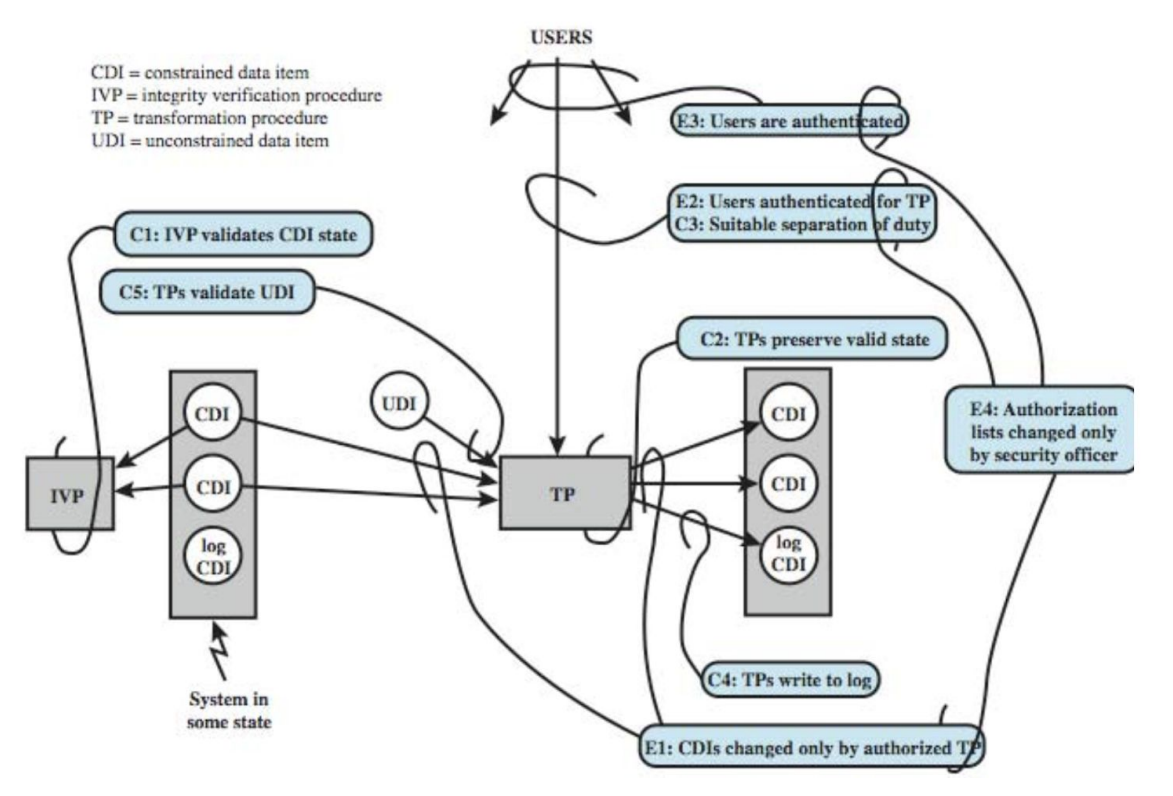
\includegraphics[width=10cm, keepaspectratio]{capitoli/policy/imgs/clark_wilson5.png}
\end{figure}

\subsubsection{I principali limiti}
\begin{itemize}
      \item Staticità delle relazioni di autorizzazione,
      \item Staticità della separazione dei compiti,
      \item Concessione centralizzata delle autorizzazioni assegnata all'
            amministratore della sicurezza.
\end{itemize}

\subsubsection{Biba vs. Clark-Wilson}
In Biba la fiducia nei soggetti viene valutata in base alle azioni
che soddisfano le regole e non in base alla nozione di regola di certificazione.
I dati non fidati
vengono esaminati prima di essere dichiarati fidati. In Clark-Wilson ci sono
degli espliciti requisiti
che regolano le azioni che possono essere fatte; inoltre le entità fidate devono
certificare il metodo
per aggiornare il dato da non fidato a fidato (e non il dato stesso).
Biba si basa sull'integrità multi-livello, mentre Clark-Wilson focalizza la
separazione dei compiti e
delle transazioni.


\section{Hybrid Policies}

Le policy ibride servono per garantire sia la confidenzialità che l'integrità.
Le principali sono: modello a Muraglia Cinese (\textbf{Chinese Wall}) basato sul
concetto di conflitto di interesse; \textbf{ORCON} che combina le regole di
controllo sugli accessi di tipo mandatory con quelle di tipo discretionary;
\textbf{RBAC} dove l'accesso avviene tramite regole di controllo basate sui
ruoli di appartenenza (usato in ambienti commerciali come SAP).

\subsection{Chinese Wall}

La politica della “\textit{muraglia cinese}” è stata introdotta da Brewer e Nash
nel 1989 per evitare che informazioni sensibili, concernenti una certa compagnia,
vengano passate a compagnie rivali per mezzo di consulenti finanziari.
Si stabiliscono dinamicamente i diritti di accesso degli utenti in base
alle risorse a cui l'utente stesso ha già avuto accesso.
Tale modello organizza le entità in classi basate su \textit{Conflitti di Interesse}.
Il controllo sull'utente
viene effettuato prima dell'accesso ad ogni classe e al momento della scrittura,
in questo ultimo
caso il controllo viene fatto su tutte le classi per avere la certezza che
l'informazione non violi le
regole sui conflitti di interesse. Per ogni classe di conflitto di interesse
saranno definite delle
informazioni visibili a tutti chiamate “\textbf{Sanitized Data}”
(informazioni prive di dati sensibili).
Occorre definire tre elementi:

\begin{itemize}
      \item \textit{Oggetti} (\textbf{O}): sono gli elementi di informazione
            relativi ad un'azienda;
      \item \textit{Company Dataset} (\textbf{CD}): contiene l'insieme degli
            oggetti relativi ad una singola azienda
            (l'operazione di inserimento di un oggetto è chiamata \(CD(o)\));
      \item \textit{Conflict of Interest Class} (\textbf{CoI}): contiene
            l'insieme delle aziende in concorrenza tra di
            loro (l'operazione di inserimento di un'azienda è detta \(CoI(o)\));
            ogni oggetto appartiene
            esattamente a una classe CoI.
\end{itemize}

Prendiamo in esame la seguente immagine:

\begin{figure}[H]
      \centering
      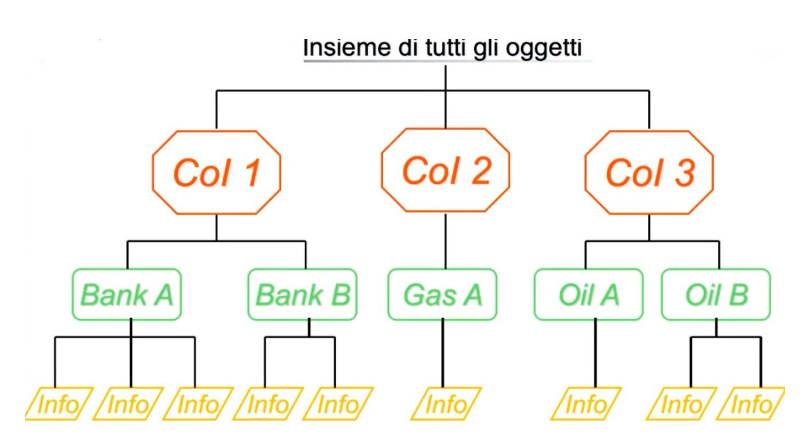
\includegraphics[width=10cm, keepaspectratio]{capitoli/policy/imgs/chinese1.png}
\end{figure}

Gli oggetti \textit{O} solo le “Info”. I \textit{CD} sono \verb|Bank A|
e \verb|Bank B|, \verb|Gas A|, \verb|Oil A| e \verb|Oil B|.
Le banche \verb|A| e \verb|B| sono
in conflitto tra loro e per questo nella
medesima \textit{CoI} indicata con 1. Gli altri CD
appartengono alle \textit{CoI} 2 e 3.
Il protocollo vuole evitare che se un
consulente accede ai dati della banca \verb|A|, non
può accedere a quelli della banca \verb|B| perché
esse sono chiaramente in conflitto.
Quindi, se un consulente legge un oggetto appartenente ad un \textit{CD} in una
data \textit{CoI}, non può più
leggere oggetti di altri \textit{CD} in quella \textit{CoI}.
È possibile che le informazioni apprese prima possano consentirgli di prendere
decisioni “migliori” dopo (ovviamente in modo sleale).
Indichiamo con \(PR(S)\) l'insieme degli oggetti che \textit{S} ha già letto.
Una semplice condizione di sicurezza in fase di lettura, prevede che un soggetto
\textit{S} può leggere un
oggetto \textit{O} se e solo se:

\begin{itemize}
      \item Esiste un oggetto \(o'\) a cui \textit{S} ha avuto accesso e
            \(CD(o') = CD(o)\) oppure
      \item Per ogni \(o' \in O, \ o' \in PR(S) \Rightarrow CoI(o') \neq CoI(o)\).
\end{itemize}

\(o\) (minuscolo) è un oggetto sanitized e perciò non genererà conflitti di
interesse.
In questa politica non vengono presi in considerazione i dati sanitized ed
inizialmente \(PR(S) = \emptyset \).
In altri termini, un soggetto può leggere un oggetto se l'oggetto è in un dataset
di cui il soggetto ha
già letto qualcosa oppure l'oggetto appartiene a una \textit{CoI} di cui il
soggetto non ha letto ancora niente. Nel nostro esempio, se il consulente legge
dalla banca \verb|A| non potrà leggere dalla \verb|B|. Non
appena viene compiuta un'azione di lettura viene negato l'accesso ad altri dati
che potrebbero generare conflitti di interessi.
La politica \textbf{Chinese Wall} è una combinazione di \textit{libera scelta} e
\textit{MAC}. Inizialmente un soggetto è
libero di accedere a ciò che vuole ma, una volta effettuata la scelta, per
quell'utente viene creata una \textit{Muraglia Cinese} attorno al dataset a cui
l'oggetto appartiene.
Si noti che la Chinese Wall può essere combinata con le politiche DAC.

\paragraph{Esempio.}
Anthony e Susan lavorano per la stessa azienda di consulenza.
Anthony può leggere i \textit{CD} di \verb|Bank A| e di \verb|Gas A| e Susan
può leggere i \textit{CD} di \verb|Bank B| e di \verb|Gas A|. Se Anthony potesse
scrivere sul \textit{CD} di \verb|Gas A|, Susan potrebbe leggerlo. Perciò,
indirettamente, potrebbe acquisire informazioni su
\verb|Bank B|, un chiaro conflitto di interesse. La regola così descritta per la
lettura non è in grado di prevenire “fughe di notizie”.\\

Quindi, in fase di scrittura, il modello deve stabilire che un soggetto \textit{S}
può scrivere un oggetto \(o\) se e solo se:

\begin{enumerate}
      \item La condizione di sicurezza in lettura permette a \textit{S} di
            leggere \(o\),
      \item Per ogni oggetto non \textit{sanitized} (quindi sensibile) \(o'\),
            se \textit{S} può leggere \(o'\), allora \(CD(o') = CD(o)\).
\end{enumerate}

In pratica \textit{S} può scrivere un oggetto se tutti gli oggetti sensibili
che può leggere appartengono allo stesso dataset. Un utente che ha letto più
\textit{CD} non potrà scrivere nessun oggetto; inoltre, una volta
che ha scritto in un \textit{CD}, potrà scrivere soltanto lì.
Così il flusso di informazioni è destinato a restare all'interno dell'azienda.
In altri termini, un
soggetto può scrivere un oggetto se lo può anche leggere e non può leggere dati
di altre compagnie.

\subsubsection{Chinese Wall vs Bell-LaPadula}

Chinese Wall non assegna etichette di sicurezza
ma si basa sugli accessi passati. Bell-LaPadula può
simulare Chinese Wall istante per istante, in questo
caso: ogni coppia di \verb|(CoI, CD)| costituirà una
categoria, ci saranno due livelli di sicurezza (\textit{S}
(sanitized), \textit{U} (non sanitized), in cui \textit{S} domina \textit{U}),
ad ogni soggetto deve essere associata al massimo
una sola categoria per ogni classe \textit{CoI}. Però,
Bell-LaPadula non sarà in grado di gestire gli
accessi passati e di adattare i vincoli relativi ai
permessi di accesso con il variare del tempo (in
Chinese Wall infatti, inizialmente si ha accesso a
tutti gli oggetti, poi no).

\subsubsection{Chinese Wall vs Clark-Wilson}

Se non è prevista una distinzione tra i soggetti
ed i processi, allora si rispetterebbe il modello
di Clark-Wilson ma si violerebbe il modello
Chinese Wall (una singola persona può
accedere a più processi). Se però è prevista
una separazione tra soggetto e processo allora
si dovrebbero rispettare entrambi i modelli in
termini di sicurezza di integrità.

\subsection{ORCON \normalfont\emoji{ogre}}

Il modello ORCON stabilisce che i diritti di accesso vengono definiti
dall'utente che ha creato l'oggetto. Il diritto di lettura di un dato non è
concesso al possessore del dato ma a colui che l'ha
originato.

\begin{enumerate}
      \item Il soggetto \(s \in S\) marca l'oggetto \(o \in O\) come ORCON per
            conto dell'organizzazione \(X\).
      \item \(X\) permette che \(o\) sia diffuso ai soggetti che lavorano per
            conto dell'organizzazione \(Y\) con le seguenti restrizioni:
            \begin{itemize}
                  \item \(o\) non può essere rilasciato a soggetti che lavorano per
                        conto di altre organizzazioni senza il permesso di \(X\);
                  \item Ogni copia di \(o\) deve avere le stesse restrizioni.
            \end{itemize}
\end{enumerate}

Per realizzare questa politica non sono idonei nè \textit{MAC} nè \textit{DAC}.
DAC non può essere utilizzato poiché il possessore potrebbe concedere qualsiasi
diritto violando la seconda proprietà.
MAC è inadeguato poiché:

\begin{itemize}
      \item può causare un'esplosione del numero di categorie;
      \item la gestione degli accessi avviene in maniera centralizzata,
            mentre in ORCON è richiesta
            una gestione locale.
\end{itemize}

La soluzione prevede la combinazione di MAC e DAC generando la seguente tecnica
di gestione degli accessi: il possessore dell'oggetto non può cambiare i
controlli di accesso. Quando l'oggetto
viene copiato, vengono copiate anche le restrizioni di accesso dalla sorgente
(cioè è MAC, il possessore non può controllarlo); il creatore del documento può
alterare le restrizioni di accesso in base al soggetto e all'oggetto
(cioè è DAC, il creatore può controllarlo).

\subsection{RBAC}

Il modello \textbf{RBAC} (\textit{Role Based Access Control}) nasce poiché un
problema importante nell'organizzazione di grandi sistemi è la complessità
dell'amministrazione della sicurezza.
Quando il numero dei soggetti e degli oggetti è alto, il numero di autorizzazioni
può diventare molto grande.
Inoltre, se l'utenza è dinamica, il numero di concessioni e di revoche di permessi
diventa davvero elevato. Gli utenti finali spesso non “possiedono” le informazioni
a cui hanno accesso. Le aziende o gli enti sono i reali possessori degli oggetti.
Il controllo di accesso è quindi basato sulle mansioni delle persone e non sul
semplice possesso.
RBAC è stato quindi proposto come alternativa al DAC e al MAC per semplificare
la gestione degli accessi e per supportare direttamente il controllo basato sui
ruoli.
I diritti di accesso dipendono dal ruolo del soggetto ma non dalla sua identità.
I ruoli rappresentano le mansioni all'interno di un'organizzazione;
le autorizzazioni sono concesse ai ruoli anziché ai
singoli utenti. Gli utenti sono perciò autorizzati semplicemente ad assumere ruoli
appropriati, acquisendo le autorizzazioni assegnate a quei ruoli.
Poiché i ruoli rappresentano le funzioni dell'organizzazione, un modello RBAC può
direttamente supportare le politiche di sicurezza proprie dell'organizzazione.
La concessione e la revoca delle
autorizzazioni alle categorie di utenti è estremamente semplificata.
I modelli RBAC sono anche detti “\textbf{policy-neutral}”.

\subsubsection{Modello RBAC-NIST}

Il modello RBAC NIST è una definizione standard di controllo di accesso basato
sui ruoli. Nel 2000, il NIST ha richiesto uno standard unificato per RBAC,
integrando il modello RBAC pubblicato nel 1992.
Il modello dispone di \textbf{tre} livelli con capacità funzionali crescenti:
\textbf{Core RBAC} (o Flat RBAC), \textbf{RBAC Gerarchico}, \textbf{RBAC Vincolato}.
Formalmente, RBAC definisce:

\begin{itemize}
      \item \textbf{Utente}: un essere umano, una macchina, un processo, o un
            agente intelligente autonomo, ecc.;
      \item \textbf{Ruolo}: una funzione nel contesto di un'organizzazione con
            una semantica associata
            secondo l'autorità e la responsabilità del ruolo;
      \item \textbf{Permesso}: modo di accesso che può essere esercitato sugli
            oggetti nel sistema.
      \item Sia gli oggetti e i modi di accesso sono dipendenti dal dominio;
      \item \textbf{Sessione}: è una particolare istanza di una connessione di
            un utente al sistema e definisce
            un sottoinsieme di ruoli attivati.
      \item Ad ogni istante, possono essere attive più sessioni differenti per
            ciascun utente.
      \item Quando un utente entra nel sistema, stabilisce una sessione e durante
            tale sessione può
            attivare un sottoinsieme dei ruoli che è autorizzato ad assumere;
      \item L'utente ottiene i permessi associati al ruolo che ha attivato nella
            sessione
\end{itemize}

\paragraph{RBAC Float.}

In questo primo modello vengono definiti solo gli elementi essenziali senza i
quali non è possibile implementare un controllo d'accesso.

\begin{itemize}
      \item il \textbf{ruolo} è un insieme di funzioni; \verb|trans(r)|
            indica le transazioni autorizzate per il ruolo \verb|r|;
      \item I ruoli attualmente attivi per il soggetto \verb|s| sono dati da
            \verb|actr(s)|;
      \item il set di ruoli autorizzati per il soggetto \verb|s| si calcolano
            con \verb|authr(s)|;
      \item le azioni che il soggetto \verb|s| può fare al tempo \verb|t| si
            ricavano da \verb|canexec(s, t)| il cui risultato
            dipende dal ruolo di \verb|s|.
\end{itemize}

Sia \verb|S| l'insieme dei soggetti e \verb|T| quello delle transazioni:
le transazioni che il soggetto può fare
dipendono dal ruolo di \verb|s|; i ruoli che \verb|s| ha attivi sono un
sottoinsieme dei ruoli autorizzati per \verb|s|.
Se \verb|t| è una transazione che il soggetto \verb|s| può eseguire, allora essa
è anche una di quelle transazioni permesse a tutti i soggetti del ruolo
ricoperto da \verb|s|.

\paragraph{RBAC Gerarchico.}
La gerarchia tra i ruoli è un modo naturale per strutturarli, riflettendo le
linee di autorità e responsabilità di un'organizzazione. Ad un ruolo
gerarchicamente più importante, saranno assegnate le stesse azioni di un ruolo
meno importante più alcune specifiche, ovvero:

\[
      (\forall s \in S)[ \ r' \in authr(s) \wedge r' > r \rightarrow r \in authr(S) \ ]
\]\footnote{È inutile ed incomprensibile, ma era carina da vedere.}

In tale modello è applicabile il principio di ereditarietà:

\begin{itemize}
      \item \textit{Ereditarietà di utente} (\textbf{UI}): Tutti gli utenti
            autorizzati ad un ruolo \verb|r| sono anche autorizzati ad
            un ruolo \verb|r'|, ove \(r > r'\)
      \item \textit{Eredità di permessi} (\textbf{PI}): Un ruolo \verb|r| è
            autorizzato a tutti i permessi per i quali ogni ruolo \verb|r'|,
            tale che \(r > r'\), è autorizzato
      \item \textit{Eredità di attivazione} (\textbf{AI}): Attivando un
            ruolo \verb|r| automaticamente si attivano tutti i ruoli \verb|r'|,
            tali che \(r > r'\).
\end{itemize}

\paragraph{RBAC Vincolato.}
È un modello RBAC con la capacità di supportare le politiche di
\textit{Separazione dei compiti}
(\textbf{Separation of Duty}). Evita conflitti di interesse e collisioni tra
mansioni.
Sia \verb|r| un ruolo e \verb|s| un soggetto tale che \verb|r|
appartiene a \verb|auth(s)|, allora il predicato
\verb|meauth(r)| (usato per assegnare autorizzazioni in mutua esclusione) è
l'insieme dei ruoli che \verb|s| non può assumere a
causa dei requisiti di separazione dei
compiti.

\[
      (\forall r_1, r_2 \in R) [ \ r_2 \in meauth(r_1) \rightarrow
                  [ \ (\forall s \in S) [ \ r_1 \in authr(s) \rightarrow r_2 \notin authr(s) \ ] \ ] \ ]
\] \footnote{Anche questa è inutile ed incomprensibile, ma carina da vedere.}

In pratica, la \textit{Separation of Duty} stabilisce che
se un ruolo \(r_2\) è in conflitto con un ruolo \(r_1\),
allora ogni soggetto \verb|s| autorizzato al ruolo \(r_1\)
non può essere autorizzato al ruolo \(r_2\).
Esistono due tipi di categorie di separazione dei compiti (Separation of Duty):

\begin{itemize}
      \item \textbf{Statici}: restringono l'insieme dei ruoli, ed in particolare
            la possibilità di entrare nella
            relazione RA. Per evitare che una persona sia autorizzata ad assumere
            troppi ruoli, nessun
            utente può assumere più di un certo numero di ruoli in un determinato
            insieme di ruoli;
      \item \textbf{Dinamici}: limitano il numero di ruoli che un utente può
            attivare in una singola sessione.
            Ad esempio si può stabilire un massimo numero di ruoli in una sessione,
            oppure si può stabilire che se assunto un ruolo in una sessione non
            si possono assumere altri ruoli nella stessa
            sessione. Ovviamente per garantire questa tecnica di assegnamento
            dei compiti, è
            importante mantenere una storia dei ruoli attivati da ciascun
            utente nell'arco della sessione.
\end{itemize}

In conclusione, le politiche ibride riguardano sia la riservatezza che l'integrità.
Diverse combinazioni di questi modelli ORCON non sono né MAC né DAC.
In realtà, un modello RBAC combinato controlla l'accesso in base alle funzionalità.